\documentclass[letterpaper,11pt]{article}

% Soporte para los acentos.
\usepackage[utf8]{inputenc}
\usepackage[T1]{fontenc}
% Idioma español.
\usepackage[spanish,mexico, es-tabla]{babel}
% Soporte de símbolos adicionales (matemáticas)
\usepackage{amsmath}
\usepackage[dvipsnames]{xcolor}
% Modificamos los márgenes del documento.                                       
\usepackage[lmargin=1.5cm,rmargin=1.5cm,top=1.5cm,bottom=1.5cm]{geometry}

\usepackage{graphicx}

\usepackage{alltt}

\title{Facultad de Ciencias, UNAM \\ 
       Lenguajes de Programación\\ 
       Tarea 6}
\author{ Rodríguez Campos Erick Eduardo\\ Rubí Rojas Tania Michelle}
\date{23 de enero de 2021}

\begin{document}

\maketitle 

\begin{enumerate}
    % Pregunta 1
    \item Evalúa el siguiente código en \textsc{Racket}, explica su resultsado, y 
    da la continuación asociada a evaluar, usando la notación $\lambda \uparrow$.
    \begin{itemize}
        \item [$>$] \texttt{(define c \#f)}
        \item [$>$] \texttt{(+ 1 (+ 2 (+ 3 (+ (let/cc k (set! c k) 4) 5))))}
        \item [$>$] \texttt{(c 10)}
    \end{itemize}
    \begin{center}
        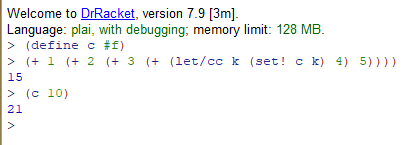
\includegraphics[scale=.9]{imagenes/rack01.PNG}
    \end{center}
    Cuando invocamos una continuación, esta nos envía de regreso al punto en el programa donde se evaluó la expresión marcada, la continuación toma un argumento, que remplaza el valor de la expresión marcada y la evaluación se reanuda a partir de ahí. 
    Tenemos que \textit{$let/cc$} hace tres cosas:
    \begin{enumerate}
        \item Sirve como la expresión marcada por la continuación.
        \item Captura la continuación ($cc$ significa ''continuación actual'') y la asigna a una variable que designamos, en este caso $k$.
        \item Como el $let$, evalúa cualquier expresión dentro y la última expresión se convierte en el valor de retorno. En este caso, $let/cc$ guarda nuestra continuación en la variable $c$, y luego devuelve $4$ (ya que $c$ tiene como valor \#f). Por lo tanto el valor de la expresión es $15$.
    \end{enumerate}
    \texttt{Notación $\lambda \uparrow$:}
    \begin{verbatim}
        (+ 1 (+ 2 (+ 3 (+ (let/cc k (set! c k) 4) 5))))
        (+ 1 (+ 2 (+ 3 (+ (lambda \uparrow (k) (k (+ 1 (+ 2 (+ 3 (+ 4 5))))))))))
        (k (+ 1 (+ 2 (+3 (+ 4 5)))))
        (k 15) = 15
    \end{verbatim}

    Cuando invocamos nuestra continuación $c$ con un argumento, es equivalente a reemplazar el valor de $4$ por el valor de $c$, y así el valor de la expresión es $21$.\\
    \newpage
    \texttt{Notación $\lambda \uparrow$:}
    \begin{verbatim}
        (+ 1 (+ 2 (+ 3 (+ (let/cc k (set! c k) 4) 5))))
        (+ 1 (+ 2 (+ 3 (+ (lambda \uparrow (k) (k (+ 1 (+ 2 (+ 3 (+ 10 5))))))))))
        (k (+ 1 (+ 2 (+3 (+ 10 5)))))
        (k 21) = 21
    \end{verbatim}
    
    %Pregunta 2
    \item Modifica cada una de las siguientes funciones de forma que usen el estilo de paso de continuaciones (Continuation Passing Style).
    \begin{itemize}
        \item [$(a)$] \begin{alltt}(define (potencia n m)
    (if (zero? m)
        1
        (* n (potencia n (sub1 m)))))
        \end{alltt}
        Modificar la función usando la técnica de recursión de cola:
        \begin{alltt}
(define (potencia n m)
    (potencia-tail n m 1))
    
(define (potencia-tail n m acc)
    (if (zero? m)
        acc
        (potencia-tail n (sub1 m) (* n acc))))
        \end{alltt}
        Transformar la función usando CPS:
        \begin{verbatim}
(define (potencia n m)
    (potencia/k n m ((lambda (x) x)))
    
(define (potencia/k n m k)
    (if (zero? m)
        (k 1)
        (potencia/k n (sub1 m) (lambda(v) (k (* n v))))))
        \end{alltt}
        \item [$(b)$] \begin{alltt}(define (suma-digitos n)
    (if (< n 10)
        n
        (+ (modulo n 10) (suma-digitos (quotient n 10)))))
        \end{alltt}
        Modificar la función usando la técnica de recursión de cola:
        \begin{alltt}
(define (suma-digitos n)
    (suma-digitos-tail n 0))
    
(define (suma-digitos-tail n acc)
    (if (= n 0)
        acc
        (sumar-digitos-tail (quotient n 10) (+ acc (modulo n 10)))))
        \end{alltt}
        Transformar la función usando CPS:
        \begin{alltt}
(define (suma-digitos n)
    (suma-digitos/k n (lambda (x) x)))
    
(define (suma-digitos/k n k)
    (if (= n 0)
        (k 0)
        (suma-digitos/k (quotient n 10) (+ lambda(v) (k (+ v (modulo n 10)))))))
        \end{alltt}
        \item [$(c)$] \begin{alltt}(define (cuadrados lst)
    (if (empty? lst)
        empty
        (cons (expt (car lst) 2) (cuadrados xs))))
        \end{alltt}
        Modificar la función usando la técnica de recursión de cola:
        \begin{alltt}
    (define (cuadrados lst)
        (cuadrados-tail lst '()))
        
    (define (cuadrados-tail lst acc)
        (if (empty? lst)
            acc
            (cuadrados-tail (cdr lst) (cons acc (expt (car lst) 2)))))
        \end{alltt}
        Transformar la función usando CPS:
        \begin{alltt}
    (define (cuadrados lst)
        (cuadrados/k lst (lambda (x) x)))
        
    (define (cuadrados/k lst k)
        (if (empty? lst)
            (k empty)
            (cuadrados/k (cdr lst) (lambda (v) (k (cons (expt (car lst) 2) v))))))
        \end{alltt}
        \item [$(d)$] \begin{alltt} (define (reversa lst)
    (if (empty? lst)
        empty
        (append (reversa (cdr lst)) (list x))))
    \end{alltt}
    Modificar la función usando la técnica de recursión de cola:
    \begin{alltt}
    (define (reversa lst)
        (reversa-tail lst '()))
        
    (define (reversa-tail lst acc)
        (if (empty? lst)
            acc
            (reversa-tail (cdr lst) (cons acc (car lst)))))
    Transformar la función usando CPS:
    \begin{alltt}
    (define (reversa lst)
        (reversa/k lst (lambda (x) x)))
        
    (define (reversa/k lst k)
        (if (empty? lst)
            (k empty)
            (reversa/k (cdr lst) (lambda (v) (k (append v (list (car lst))))))))
    \end{alltt}
    \end{verbatim}
    
    \end{itemize}
    
    %Pregunta 3
    \item Evalúa la siguiente expresión usando el paso de parámetros que se indica.
    \begin{verbatim}
        {with {{a 8}
               {b -8}
               {swap {fun {x y}
                        {with {{tmp x}}
                           {seqn {set x y}
                                  {set y tmp}}}}}}
           {seqn {swap a b}
                 {- a {+ b a}}}}
    \end{verbatim}
    \begin{itemize}
        \item [$(a)$] Paso de parámetros por valor.\\
        Ambiente:
        \begin{center}
            \begin{tabular}{|l| c }
            \cline{1-1}
                \texttt{swap \hspace{1cm} \{fun \{x y\}
                        \{with \{\{tmp x\}\}
                           \{seqn \{set x y\}
                                  \{set y tmp\}\}\}\}} & 0x12\\\cline{1-1}
                \texttt{b \hspace{1.58cm} -8} & 0x11\\\cline{1-1}
                \texttt{a \hspace{1.6cm} 8} & 0x10\\\cline{1-1}
            \end{tabular}
        \end{center}
        Evaluación de \texttt{\{swap a b\}}:        \begin{verbatim}
            {{fun {x y} {with {{temp x}} seqn {set x y} {set y temp}}} 8 -8}
            {with {{temp 8}} {seqn {set x -8} {set y tmp}}}
            {seqn {set x -8} {set y 8}}
            {set x -8}      entonces x = -8
            {set y 8}       entonces y = 8
        \end{verbatim}
        Evaluación de \texttt{\{-a \{+ b a\}\}}:
        \begin{verbatim}
            {- 8 {+ b 8}}
            {- 8 {+ -8 8}}
            {- 8 {0}} = 8
        \end{verbatim}
        \item [$(b)$] Paso de parámetros por referencia.\\
        Ambiente:
        \begin{center}
            \begin{tabular}{|l| c }
            \cline{1-1}
                \texttt{swap \hspace{1cm} \{fun \{x y\}
                        \{with \{\{tmp x\}\}
                           \{seqn \{set x y\}
                                  \{set y tmp\}\}\}\}} & 0x12\\\cline{1-1}
                \texttt{b \hspace{1.58cm} -8} & 0x11\\\cline{1-1}
                \texttt{a \hspace{1.6cm} 8} & 0x10\\\cline{1-1}
            \end{tabular}
        \end{center}
        Evaluación de \texttt{\{swap a b\}}:        \begin{verbatim}
            {{fun {x y} {with {{temp x}} seqn {set x y} {set y temp}}} 8 -8}
            {with {{temp 8}} {seqn {set x -8} {set y tmp}}}
            {seqn {set x -8} {set y 8}}
            {set x -8}      entonces x = -8
            {set y 8}       entonces y = 8
        \end{verbatim}
        Ambiente modificado:
        \begin{center}
            \begin{tabular}{|l| c }
            \cline{1-1}
                \texttt{swap \hspace{1cm} \{fun \{x y\}
                        \{with \{\{tmp x\}\}
                           \{seqn \{set x y\}
                                  \{set y tmp\}\}\}\}} & 0x12\\\cline{1-1}
                \texttt{b \hspace{1.58cm} 8} & 0x11\\\cline{1-1}
                \texttt{a \hspace{1.6cm} -8} & 0x10\\\cline{1-1}
            \end{tabular}
        \end{center}
        Evaluación de \texttt{\{-a \{+ b a\}\}}:
        \begin{verbatim}
            {- -8 {+ b -8}}
            {- -8 {+ 8 -8}}
            {- -8 {0}} = -8
        \end{verbatim}
    \end{itemize}
    
    %Pregunta 4
    \item Evalúa la siguiente expresión usando el paso de parámetros que se indica.
    \begin{verbatim}
        {with {{a 1}
               {foo {fun {x}
                       {seqn {set a {+ {* x -2} a}}
                       a}}}}
           {{fun {y} {+ y {- y y}} {foo 3}}}}
    \end{verbatim}
    \begin{itemize}
        \item [$(a)$] Paso de parámetros por nombre.\\
        Ambiente:
        \begin{center}
            \begin{tabular}{|l| c }
            \cline{1-1}
                \texttt{foo \hspace{1cm} \{fun \{x\} \{seqn \{set a \{+ \{* x -2\} a\}\} a\}\}} & 0x11\\\cline{1-1}
                \texttt{a \hspace{1.4cm} 1} & 0x10\\\cline{1-1}
            \end{tabular}
        \end{center}
        Evaluación de \texttt{\{\{fun \{y\} \{+ y \{- y y\}\}\} \{foo 3\}\}}:
        \begin{verbatim}
            {+ {foo 3} {- {foo 3} {foo 3}}}
        \end{verbatim}
        Evaluación de la primera ocurrencia de \texttt{\{foo 3\}}:
        \begin{verbatim}
            {{fun {x} {seqn {set a {+ {* x -2} a}} a}} 3}
            {seqn {set a {+ {* 3 -2} a}} a}
            {set a {+ -6 1}}     entonces a = -5
        \end{verbatim}
        Ambiente modificado:
        \begin{center}
            \begin{tabular}{|l| c }
            \cline{1-1}
                \texttt{foo \hspace{1cm} \{fun \{x\} \{seqn \{set a \{+ \{* x -2\} a\}\} a\}\}} & 0x11\\\cline{1-1}
                \texttt{a \hspace{1.4cm} -5} & 0x10\\\cline{1-1}
            \end{tabular}
        \end{center}
        Evaluación de la segunda ocurrencia de \texttt{\{foo 3\}}:
        \begin{verbatim}
            {{fun {x} {seqn {set a {+ {* x -2} a}} a}} 3}
            {seqn {set a {+ {* 3 -2} a}} a}
            {set a {+ -6 -5}}     entonces a = -11
        \end{verbatim}
        Ambiente modificado:
        \begin{center}
            \begin{tabular}{|l| c }
            \cline{1-1}
                \texttt{foo \hspace{1cm} \{fun \{x\} \{seqn \{set a \{+ \{* x -2\} a\}\} a\}\}} & 0x11\\\cline{1-1}
                \texttt{a \hspace{1.4cm} -11} & 0x10\\\cline{1-1}
            \end{tabular}
        \end{center}
        Evaluación de la tercera ocurrencia de \texttt{\{foo 3\}}:
        \begin{verbatim}
            {{fun {x} {seqn {set a {+ {* x -2} a}} a}} 3}
            {seqn {set a {+ {* 3 -2} a}} a}
            {set a {+ -6 -11}}     entonces a = -17
        \end{verbatim}
        Ambiente modificado:
        \begin{center}
            \begin{tabular}{|l| c }
            \cline{1-1}
                \texttt{foo \hspace{1cm} \{fun \{x\} \{seqn \{set a \{+ \{* x -2\} a\}\} a\}\}} & 0x11\\\cline{1-1}
                \texttt{a \hspace{1.4cm} -17} & 0x10\\\cline{1-1}
            \end{tabular}
        \end{center}
        Evaluamos \texttt{\{+ \{foo 3\} \{- \{foo 3\} \{foo 3\}\}\}} con los resultados de las evaluaciones de cada ocurrencia de \texttt{\{foo 3\}}:
        \begin{verbatim}
            {+ -5 {- -11 -17}}
            {+ -5 6} = 1
        \end{verbatim}
        \item [$(b)$] Paso de parámetros por necesidad.\\
        Ambiente:
        \begin{center}
            \begin{tabular}{|l| c }
            \cline{1-1}
                \texttt{foo \hspace{1cm} \{fun \{x\} \{seqn \{set a \{+ \{* x -2\} a\}\} a\}\}} & 0x11\\\cline{1-1}
                \texttt{a \hspace{1.4cm} 1} & 0x10\\\cline{1-1}
            \end{tabular}
        \end{center}
        Evaluación de \texttt{\{\{fun \{y\} \{+ y \{- y y\}\}\} \{foo 3\}\}}:
        \begin{verbatim}
            {+ {foo 3} {- {foo 3} {foo 3}}}
        \end{verbatim}
        Evaluación de la primera ocurrencia de \texttt{\{foo 3\}}:
        \begin{verbatim}
            {{fun {x} {seqn {set a {+ {* x -2} a}} a}} 3}
            {seqn {set a {+ {* 3 -2} a}} a}
            {set a {+ -6 1}}     entonces a = -5
        \end{verbatim}
        Evaluamos \texttt{\{+ \{foo 3\} \{- \{foo 3\} \{foo 3\}\}\}} con el resultado de la evaluación de \texttt{\{foo 3\}}:
        \begin{verbatim}
            {+ -5 {- -5 -5}}
            {+ -5 0} = -5
        \end{verbatim}
    \end{itemize}
    
    %Pregunta 5
    \item Evalúa la siguiente expresión usando el paso de parámetros por referencia-regreso
    \begin{verbatim}
        {with {{b 2}
               {f {fun {x} {seqn {set x 4}
                                 {+ x b}}}}}
           {+ {f b} b}}
    \end{verbatim}
    Ambiente:
    \begin{center}
        \begin{tabular}{|l| c }
        \cline{1-1}
            \texttt{f \hspace{1cm} \{fun \{x\} \{seqn \{set x  4\} \{+ x b\}\}\}} & 0x11\\\cline{1-1}
            \texttt{b \hspace{1.4cm} 2} & 0x10\\\cline{1-1}
        \end{tabular}
    \end{center}
    Evaluación de \texttt{\{f b\}}
    \begin{verbatim}
        {{fun {x} {seqn {set x 4} {+ x b}}} b}
        {seqn {set x 4} {+ x b}}    entonces x = 4
        {+ 4 b}
        {+ 4 2} = 6
    \end{verbatim}
    Ambiente modificado:
    \begin{center}
        \begin{tabular}{|l| c }
        \cline{1-1}
            \texttt{f \hspace{1cm} \{fun \{x\} \{seqn \{set x  4\} \{+ x b\}\}\}} & 0x11\\\cline{1-1}
            \texttt{b \hspace{1.4cm} 4} & 0x10\\\cline{1-1}
        \end{tabular}
    \end{center}
    Evaluación de \texttt{\{+ \{f b\} b\}\}} con el resultado de la evaluación de \texttt{\{ f b\}}:
    \begin{verbatim}
        {+ 6 b}
        {+ 6 4} = 10
    \end{verbatim}
    
    %Pregunta 6
    \item Dada la siguiente del definición del predicado primo? que decide si un número positivo mayor a $2$ es primo. Modifícala usando memoización.
    \begin{verbatim}
        (define (primo? n)
           (if (equal? n 2)
                #t
                (aux n 2 (sub1 n))))
    \end{verbatim}
    \begin{verbatim}
        (define (aux n i j)
           (cond 
              [(> i j) #t]
              [(zero? (modulo n i)) #f]
              [else (aux n (add1 i) j)]))
    \end{verbatim}
    Modificación usando memoización:
    \begin{verbatim}
        (define tbl (make-hash (list '(2 #t))))
        
        (define (primo? n)
            (primo-nemo? n 2 (sub1 n) tbl/h))
            
        (define (primo-nemo? n i j tbl/h)
            (let ([busqueda (hash-ref! tbl/h n 'vacia)])
                (match busqueda
                    [(list z) z]
                    ['vacia #:when (> i j) #t]
                    ['vacia #:when (zero? (modulo n i)) #f]
                    [else (let ([nuevo (primo-nemo? n (addl i) j tbl/h)]) 
                            (hash-set! tbl/h n nuevo) nuevo)])))
    \end{verbatim}
\end{enumerate}

\end{document}
